% This file demonstrates the use of the `article` option with the NREL style file.
% see main.tex for more details.
% ---------------
% PREAMBLE
% ---------------
\documentclass[article]{nrel}

% -----------------------------------
% DOCUMENT PROPERTIES
% -----------------------------------
\title{Writing NREL documents using LaTeX}
\author{A. Clifton, M. Dennis, A. Platt, P. Fleming, M. Lawson}
\addbibresource{files/bibliography.bib}

% -------------------------------------
% DOCUMENT STARTS HERE
% -------------------------------------
\begin{document}
\frontmatter
\mainmatter
\tableofcontents
\listoffigures
\listoftables
\clearpage
\lstset{language=[LaTeX]Tex,columns=fullflexible,keepspaces=true,breaklines=true}
\section{What is LaTeX?}
\section{Requirements for NREL documents}
\section{Using LaTeX to make documents that meet NREL's requirements}

\subsection{Floats}
Floats are images, tables or other pieces of the document that are free to move to the best place in the document for them. The two most common floats are the tabular environment (for tables) and the figure environment for figures.

\subsubsection{Tables}
Use the \texttt{tabular} environment to produce basic tables. Table~\ref{tab:widgets} is produced using this code: 

\begin{lstlisting}
\begin{table}[!h]
\centering
\caption{An example table.}\label{tab:widgets}
\begin{tabular}{lr}
Item & Quantity \\
\hline
Widgets & 42 \\
Gadgets & 13
\end{tabular}
\end{table}
\end{lstlisting}

\begin{table}[!h]
\centering
\caption{An example table.}\label{tab:widgets}
\begin{tabular}{lr}
Item & Quantity \\
\hline
Widgets & 42 \\
Gadgets & 13
\end{tabular}
\end{table}

\begin{figure*}[htp]
\centering
\hfill
\subfigure[Wind turbines at the Forward Wind Energy Center in Fond du Lac and Dodge Counties, Wisconsin. (Photo by Ruth Baranowski / NREL)\label{fig:21206}]{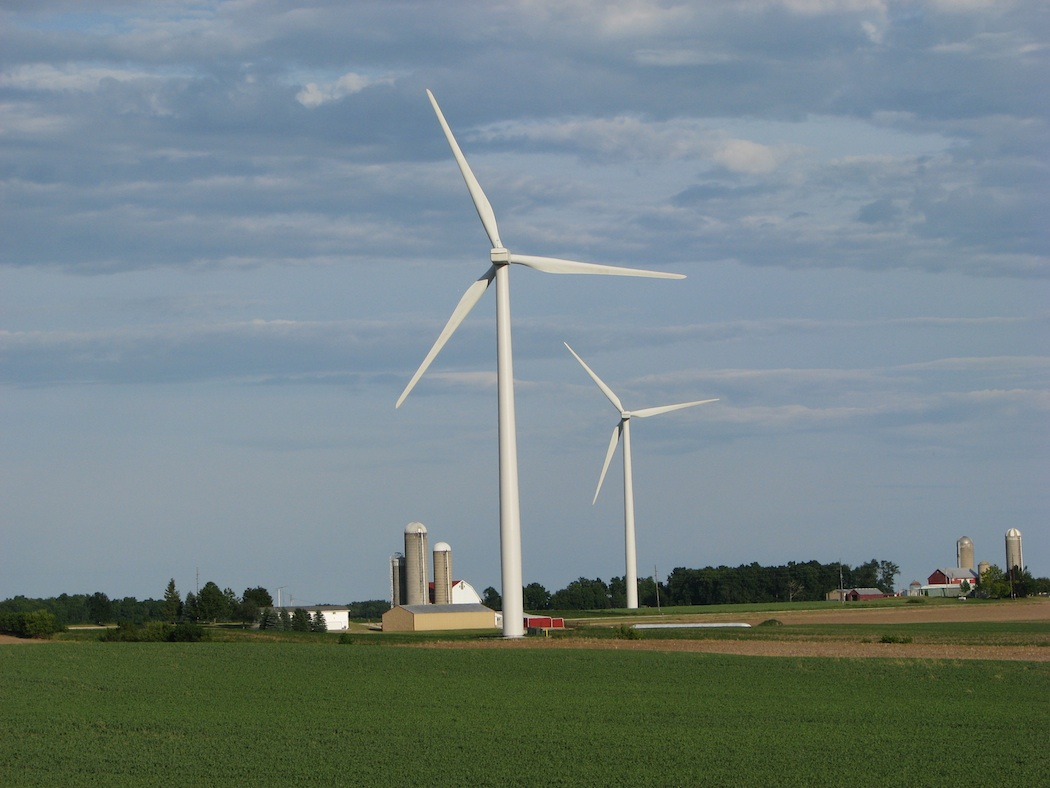
\includegraphics[height=2.5in]{files/21206}}
~ 
\hfill
\subfigure[Aerial view of the National Wind Technology Center. (Photo by Dennis Schroeder / NREL)\label{fig:20018}]{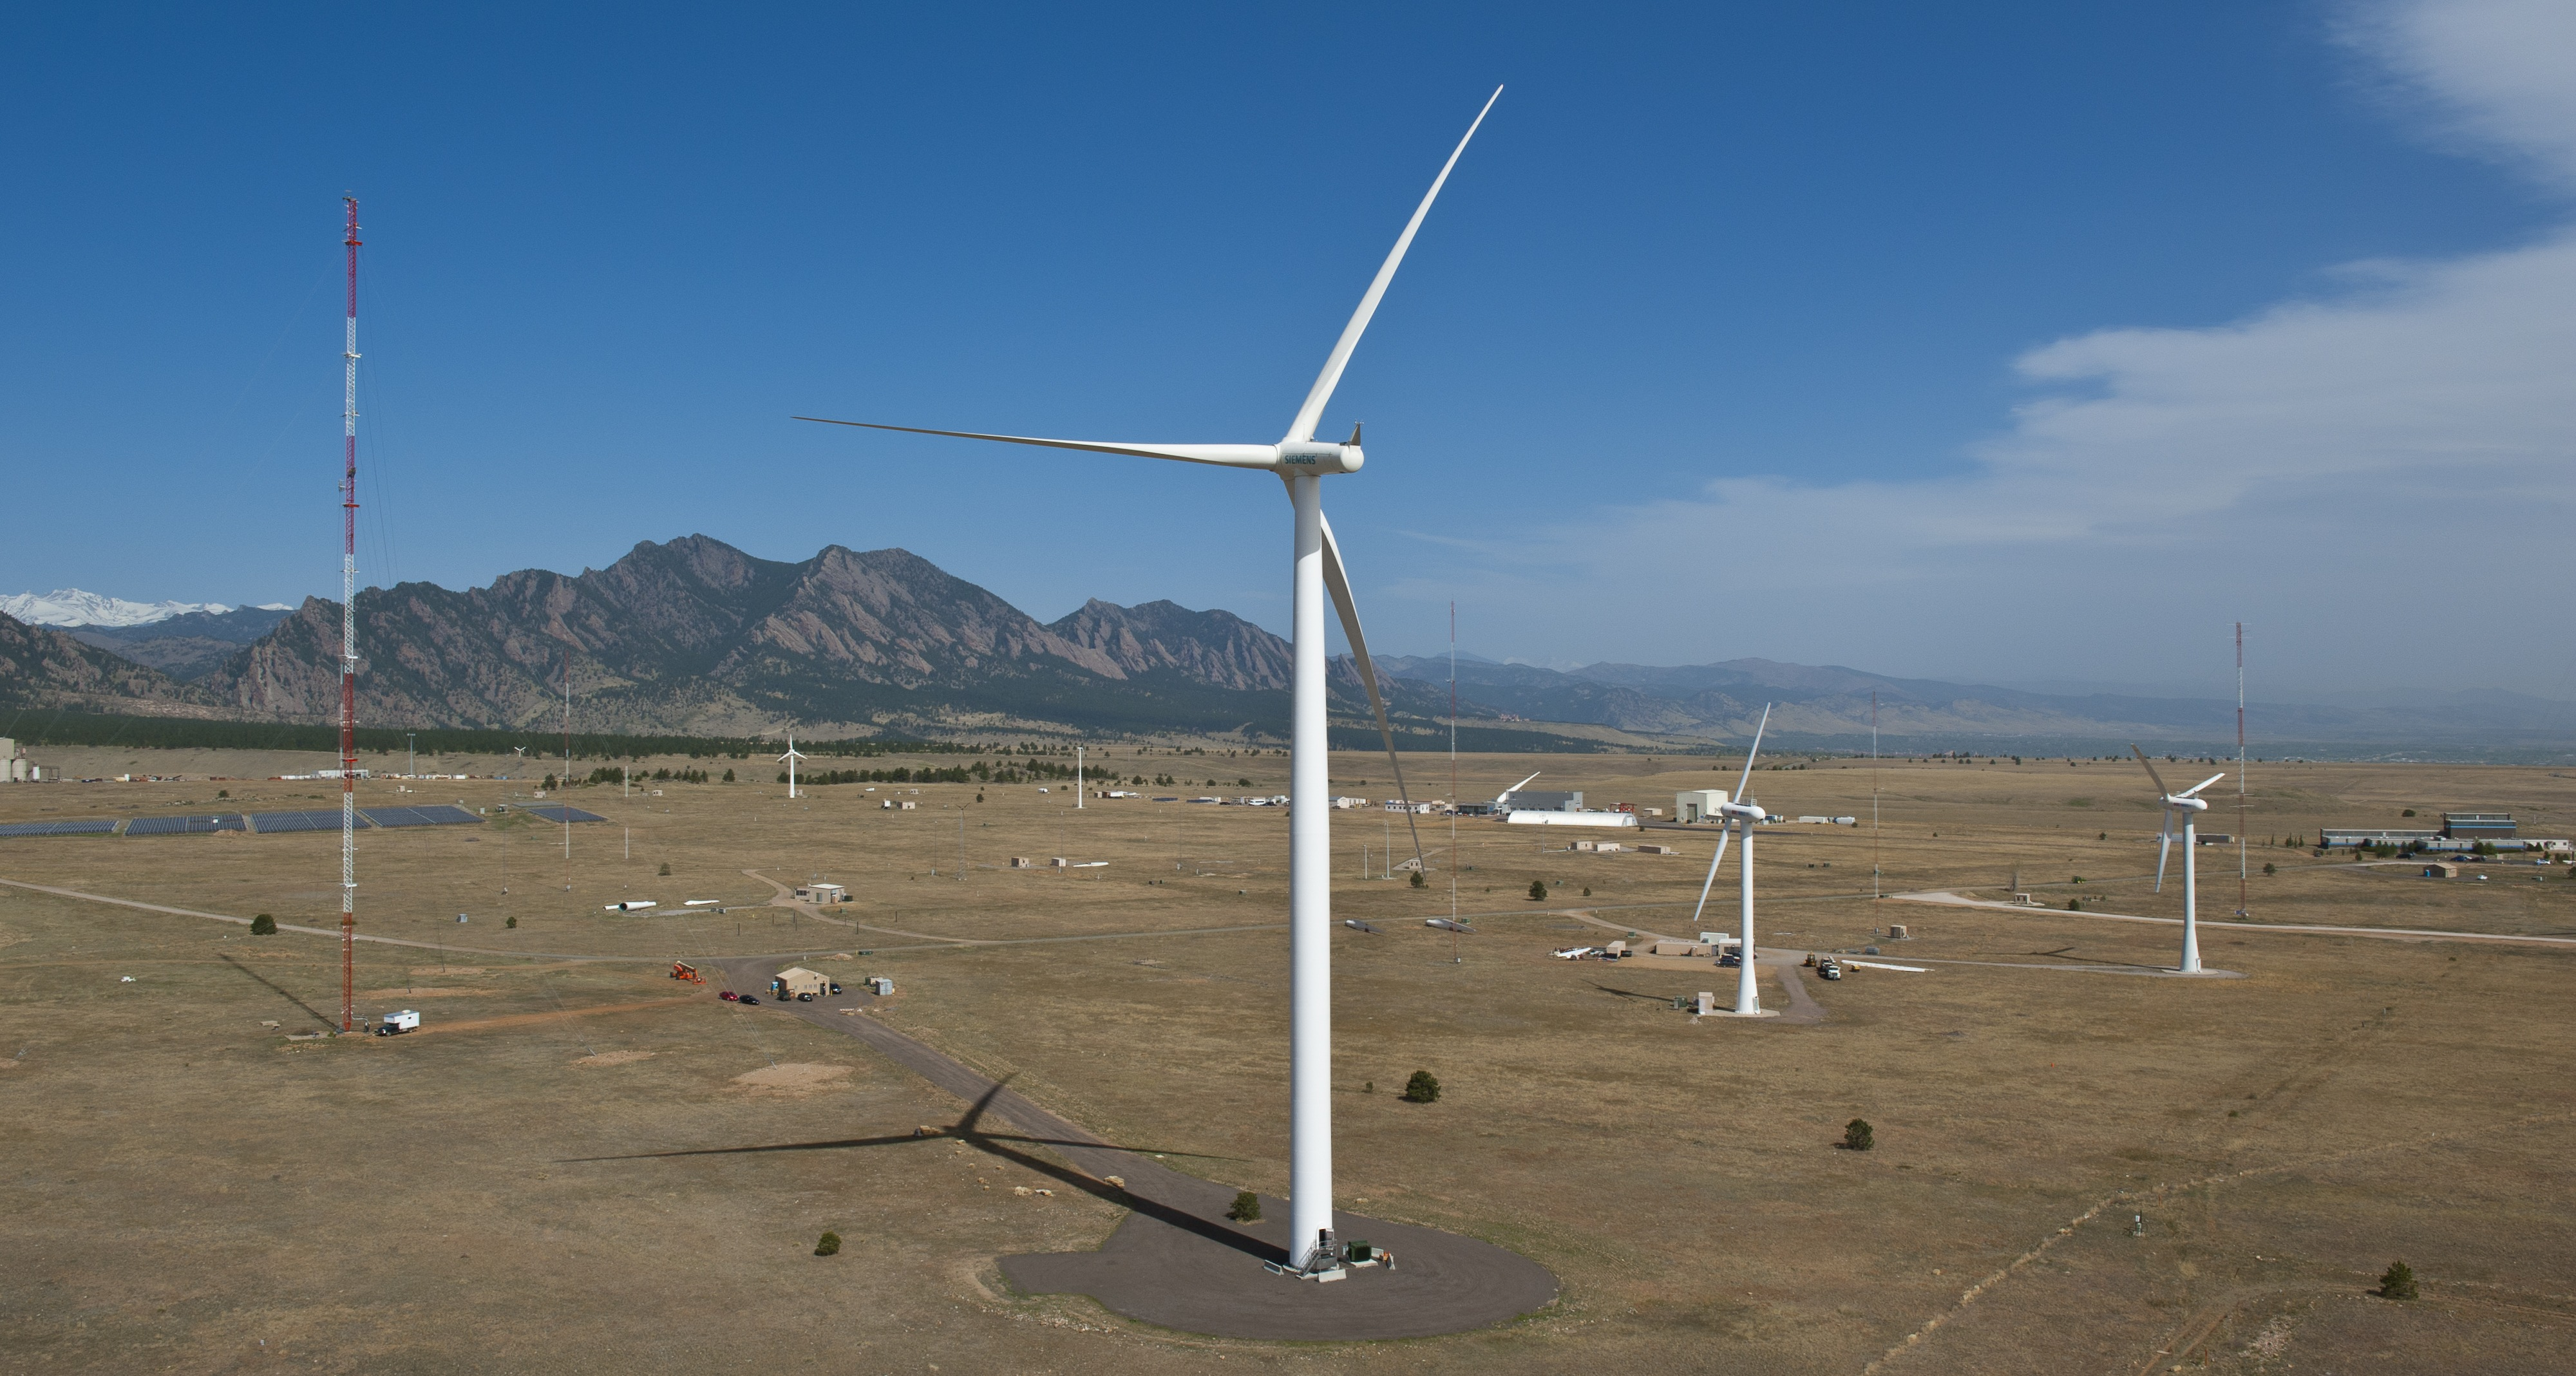
\includegraphics[height=2.5in]{files/20018}}
\hfill
\caption{NREL images}\label{fig:NRELimages}
\end{figure*}

\section{Preparing a high-quality PDF from LaTeX}
\citet{Lamport_1986_a}

% bibliography
\clearpage
\label{sec:Bib}
\printbibliography
\end{document}